\chapter{Ein Steganografischer Algorihtmus}
Die Steganografie bezeichnet eine weitere Methode die Vertraulichkeit eines
Informationsaustausches zu gewährleisten.
Es wird das Ziel verfolgt, eine Nachricht in einer für den Computer
zugänglichen Trägerdatei (engl. \textit{cover media}) zu verstecken, sodass eine
weitere Person die Existenz
einer geheimen Botschaft gar nicht erst vermuten würde. Trägerdateien, unempfindlich
gegenüber kleinen Änderungen in den Daten eignen sich besonders gut für die
Anwendung steganografischer Verfahren. Digitale Bilddateien sowie Audio- und Videodateien
sind sehr gute Trägermedien,
da ihre Daten ein ganz natürliches Rauschen aufweisen.
In diesem Kapital soll ein Algorithmus vorgestellt werden, welcher
eine beliebig lange Nachricht in einem Bild versteckt und dabei versucht,
die visuelle Qualität des Urbilds zu bewahren.
Zusätzlich wird auf eine Anwendung eingegangen, welche die beschriebenen
Ideen umgesetzt und einen Nachrichtenaustausch über
in Bildern versteckten Informationen ermöglicht.

\section{Modifikation von Bilddateien}
Eine digitale Bilddatei besteht aus einer zweidimensionalen Anordnung von Pixel, wobei
jeder eine bestimmte Farbe annehmen kann. Farben können unterschiedlich
dargestellt werden, dass in der Bildwiedergabe am häufigsten verwendete Modell ist
der RGB-Farbraum. Die Farbwahrnehmung des menschlichen Auges kann durch
das additive Mischen der drei Grundfarben Rot, Grün und Blau (RGB)
nachgebildet werden \parencite[32-40]{BOOK:VC}. In computerorientierten Anwendungen
werden hierfür pro Farbkanal Zahlenwerte zwischen 0 und 255 gespeichert,
es gilt je größer der Wert desto heller die Farbe. Die Kombinationen
$(255,0,0)$, $(0,255,0)$ und $(0,0,255)$ beschreiben jeweils die Grundfarben Rot, Grün und Blau.
Das Mischen aller Farben $(255,255,255)$ ergibt die Farbe Weiß und das Hinzufügen
gar keines Lichts $(0,0,0)$ resultiert in Schwarz. Kombinationen mit gleicher Intensität
$(100,100,100)$ werden als Grauton wahrgenommen. Pro Pixel müssen in einem Bild
also drei Byte an Information gespeichert werden, dies verspricht ein großes
Potenzial, wenn es darum geht, unentdeckt Information zu verbergen. Ein
einfaches und effektives Verfahren ist das Überschreiben der niederwertigsten
Bit (engl. \ac{lsb}) im Farbkanal
durch das zu versteckende Signal. Das Anpassen
der \acs{lsb} verändert den Farbwert nur minimal und
die kleinen Änderungen in den Zahlen werden nur durch das
Betrachten des veränderten Bilds nicht zu erkennen sein.

\paragraph{Wie stark kann ein Bild angepasst werden?}
Es soll nun abgeschätzt werden, wie stark ein Bild verändert
werden kann, ohne dass die Qualität des Ergebnisses sichtbar beeinflusst
wird. Es seien $b_7\,b_6\, \ldots \,b_0$ die acht Bit eines Farbkanals, es soll für
jeden Kanal der maximale Fehler betrachtet werden, welcher entstehen kann,
wenn die $n$ niederwertigsten Bit durch eine Nachricht ersetzt werden.
Der neue Farbwert einschließlich Fehler wird nach \eqref{eq:bit-max-error} in Bezug auf $n$ bestimmt:

\begin{equation}
  a(n) = \sum_{i=0}^{n - 1} b_i \cdot 2^i \qquad
  b_{i, n} =
  \begin{cases}
    b_i & \text{wenn $i \geq n$}                                                           \\
    1   & \text{wenn $a(n) \leq \lfloor \frac{1}{2} \cdot \sum_{i=0}^{n - 1} 2^i$} \rfloor \\
    0   & \text{sonst}
  \end{cases}
  \label{eq:bit-max-error}
\end{equation}

\noindent
\autoref{fig:peppers} zeigt die Auswirkung der Veränderung auf die Bildqualität
eines Farbbilds für Fehlerparameter $0 \leq n \leq 8$.
Es kann die durchaus vielversprechende Beobachtung
gemacht werden, dass Änderungen bis hin zur vierten Stelle im Farbkanal nur schwer und
ohne Vergleich mit der Originaldatei wahrscheinlich nicht erkannt werden würden.
\newpage

\begin{figure}[h!]
  \centering
  \begin{minipage}[t]{0.3\textwidth}
    \includegraphics[width=1\textwidth]{peppers-0.png}
    \caption*{Original ($n = 0$)}
  \end{minipage}
  \hfill
  \begin{minipage}[t]{0.3\textwidth}
    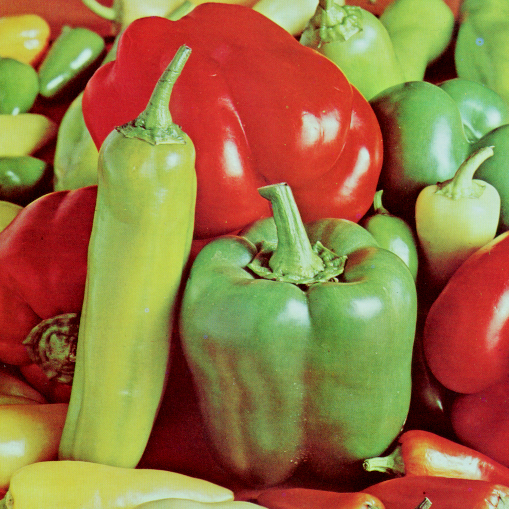
\includegraphics[width=1\textwidth]{peppers-1.png}
    \caption*{$n = 1$}
  \end{minipage}
  \hfill
  \begin{minipage}[t]{0.3\textwidth}
    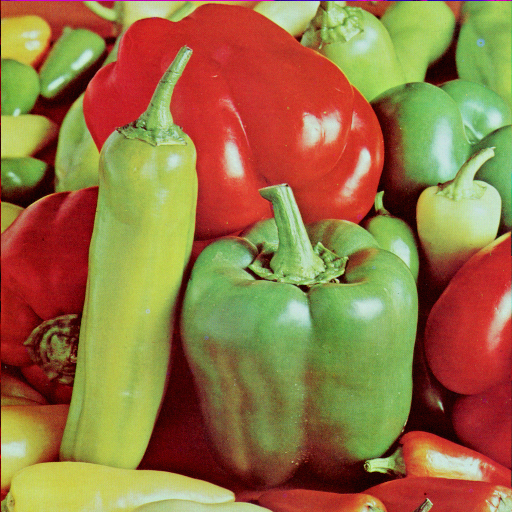
\includegraphics[width=1\textwidth]{peppers-2.png}
    \caption*{$n = 2$}
  \end{minipage}%
  \vspace{0.5cm}
  \begin{minipage}[t]{0.3\textwidth}
    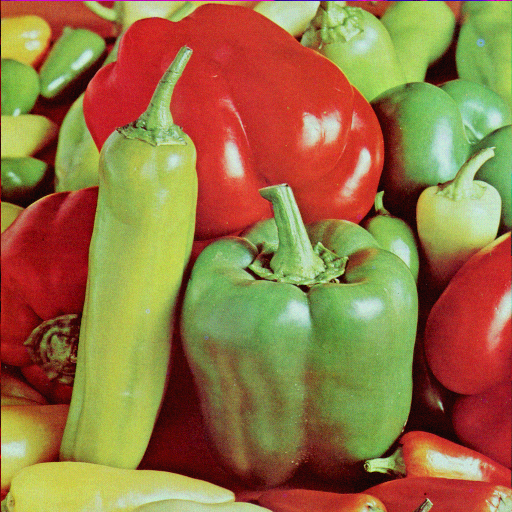
\includegraphics[width=1\textwidth]{peppers-3.png}
    \caption*{$n = 3$}
  \end{minipage}
  \hfill
  \begin{minipage}[t]{0.3\textwidth}
    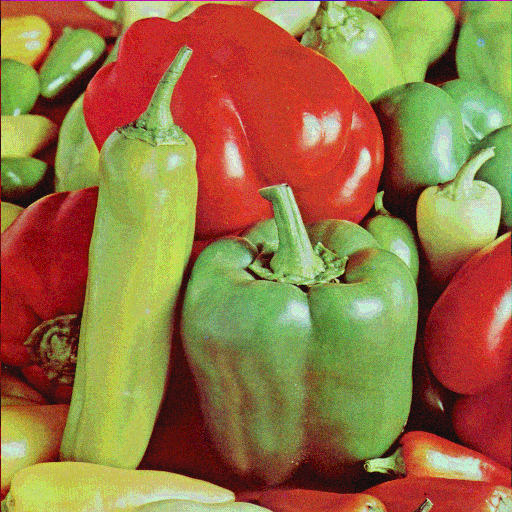
\includegraphics[width=1\textwidth]{peppers-4.png}
    \caption*{$n = 4$}
  \end{minipage}
  \hfill
  \begin{minipage}[t]{0.3\textwidth}
    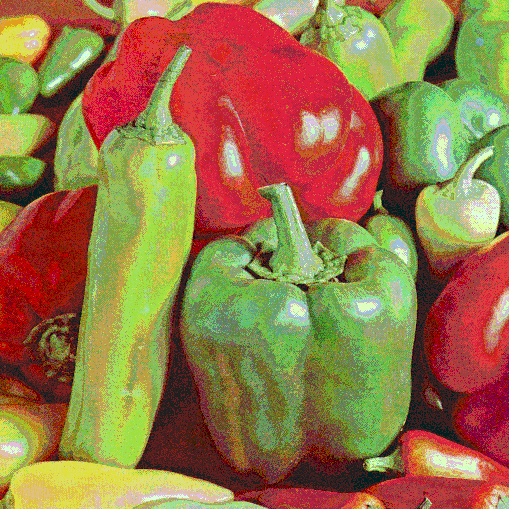
\includegraphics[width=1\textwidth]{peppers-5.png}
    \caption*{$n = 5$}
  \end{minipage}%
  \vspace{0.5cm}
  \begin{minipage}[t]{0.3\textwidth}
    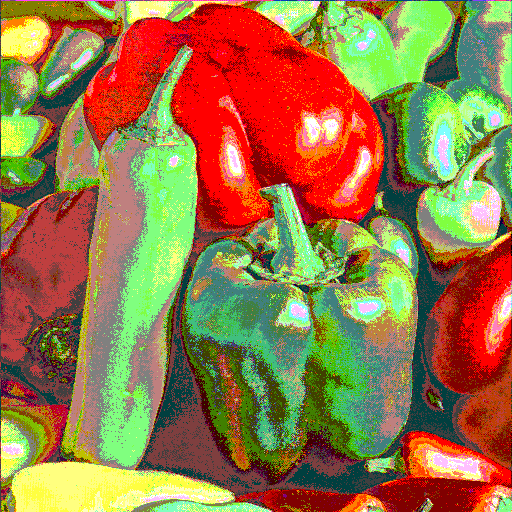
\includegraphics[width=1\textwidth]{peppers-6.png}
    \caption*{$n = 6$}
  \end{minipage}
  \hfill
  \begin{minipage}[t]{0.3\textwidth}
    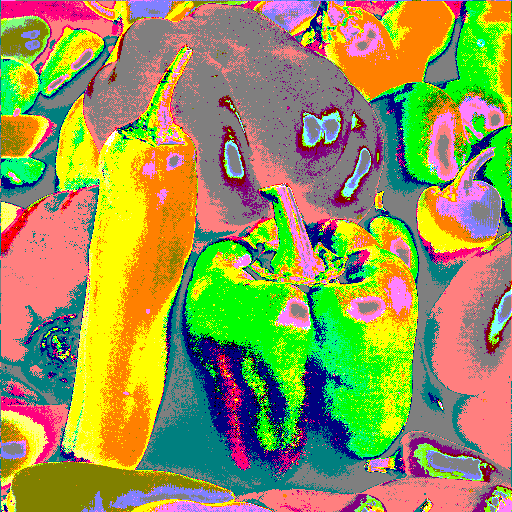
\includegraphics[width=1\textwidth]{peppers-7.png}
    \caption*{$n = 7$}
  \end{minipage}
  \hfill
  \begin{minipage}[t]{0.3\textwidth}
    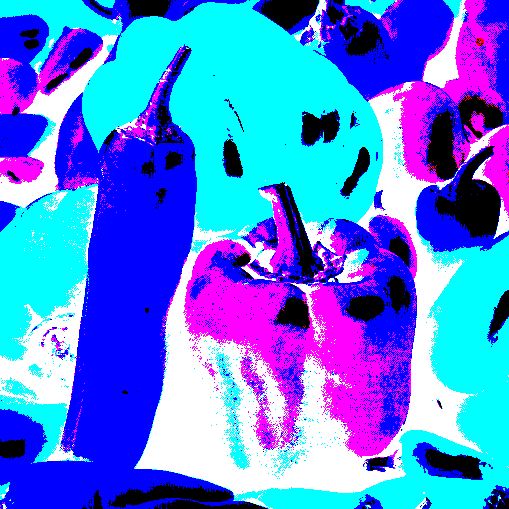
\includegraphics[width=1\textwidth]{peppers-8.png}
    \caption*{$n = 8$}
  \end{minipage}
  \caption{Farbbild Paprika verändert durch maximalen Fehler für $n \in [0,8]$.}
  \label{fig:peppers}
\end{figure}
\noindent
Zusätzlich wird in diesem Beispiel der schlimmste Fall betrachtet.
Das Verstecken einer echten Nachricht wird fast immer
ein besseres Ergebnis liefern, da Nachrichtenbit
zufällig mit den des Bilds überstimmen oder vorherige Fehler
durch weitere Teile der Nachricht wieder ausgeglichen werden.

\section{Beschreibung eines Algorithmus}
Im vorherigen Abschnitt wurden die Möglichkeiten von \acs{lsb}-Verfahren untersucht,
es kann jetzt eine mehr formale Beschreibung gegeben werden,
wie ein solcher Algorithmus umgesetzt werden kann.
Da ein steganografisches Verfahren die Vertraulichkeit einer Nachricht
nur indirekt sichert, ist es sinnvoll, diese vor dem Verwenden mit einem
kryptografischen Algorithmus zu verschlüsseln.

\begin{definition}[\acs{lsb}-Verfahren]
  Es sei $p_{xy} = (r,g,b)$ ein Pixel und $\mathbf{B} = p^{m \times n}$ ein Bild
  mit $y \in [1, m]$ und $x \in [1, n]$. Es sei $P$ die Menge aller Pixel von $\mathbf{B}$
  und $v$ eine Funktion mit $v: P \setminus \{p_{1,1},p_{mn}\} \leftarrow v(\mathbf{B})$.
  \autoref{alg:lsb-enkodierung} und \ref{alg:lsb-dekodierung} zeigen ein Verfahren für das
  Schreiben und Lesen einer Nachricht in $\mathbf{B}$.
  \begin{algorithm}
    \DontPrintSemicolon
    \KwIn{$\mathbf{B}$ und Nachricht $x$}
    \KwOut{$\mathbf{B}$ mit versteckter Nachricht $y$}
    \Begin(){
      $y \leftarrow e_k(x)$\;
      $n \leftarrow 1$\;
      schreibe Nachrichtenlänge von $y$ nach $p_{11}$ und $p_{mn}$\;
      \While(){true}{
        \lIf(){$n = 9$}{$y$ ist zu lang}
        \For{$p \in v(\mathbf{B})$}{
          \For(\tcp*[f]{Farbwerte r,g,b}){$c \in p$}{
            $b \leftarrow$ lese nächstes Bit von $y$\;
            schreibe $b$ nach Position $n$ von $c$\;
            \lIf(){$y$ bearbeitet}{\Return{}}
          }
        }
        $n \leftarrow n + 1$\;
      }
    }
    \caption{\acs{lsb}-Verfahren Schreiben}
    \label{alg:lsb-enkodierung}
  \end{algorithm}

  \begin{algorithm}[H]
    \DontPrintSemicolon
    \KwIn{$\mathbf{B}$ mit versteckter Nachricht $y$}
    \KwOut{Nachricht $x$}
    \Begin(){
      $n \leftarrow 1$\;
      $y \leftarrow \emptyset$\;
      $l \leftarrow$ lese Nachrichtenlänge bei $p_{11}$ und $p_{mn}$\;
      \While(){$l \neq 0$}{
        \For(){$p \in v(\mathbf{B})$}{
          \For(\tcp*[f]{Farbwerte r,g,b}){$c \in p$}{
            $b \leftarrow$ lese Bit bei Position $n$ von $c$\;
            $y \leftarrow y \cup \{b\}$\;
            \lIf(){$l = 0$} {
              \Return{$d_k(y)$}
            }
            \lElse(){$l \leftarrow l - 1$}
          }
        }
        $n \leftarrow n + 1$\;
      }
    }
    \caption{\acs{lsb}-Verfahren Lesen}
    \label{alg:lsb-dekodierung}
  \end{algorithm}
\end{definition}

\noindent
Damit eine Nachricht im Bild möglichst wenig auffällt, macht es Sinn, Pixel
so auszuwählen, dass diese gleichmäßig verteilt sind. Die Verteilfunktion $v$ hat genau diese
Aufgabe. Das Bild $\mathbf{B}$ wird als Folge der natürlichen Zahlen
$a = 0,1,\ldots,mn - 1$ betrachtet. Durch Wiederholtes halbieren von $a$ und
speichern der entstehenden Hälften in einer Warteschlange kann die Folge nach
dem Prinzip der Breitensuche abgearbeitet werden und es entstehen relativ gleichmäßig
verteile Koordinaten.
\begin{example}
  Ein wird ein $3 \times 3$ großes Bild betrachtet und die Zahlenfolge ist
  $a = 0,1,2,3,4,5,6,7,8$. Die nachfolgende Tabelle zeigt den Verlauf des Algorithmus:
  \begin{center}
    \begin{tabular}{cccc}
      \multicolumn{1}{c}{Warteschlange} & Mitte & Umformung           & Koordinate \\
      $[0,8]$                           & $m$   & $m = y \cdot 3 + x$ & $(x,y)$    \\
      $[5,8],[0,3]$                     & 4     & $4 = 1 \cdot 3 + 1$ & $(1,1)$    \\
      $[2,3],[0,0],[5,8]$               & 1     & $1 = 0 \cdot 3 + 1$ & $(1,0)$    \\
      $[7,8],[5,5],[2,3],[0,0]$         & 6     & $6 = 2 \cdot 3 + 0$ & $(0,2)$    \\
      $[7,8],[5,5],[2,3]$               & 0     & $0 = 0 \cdot 3 + 0$ & $(0,0)$    \\
      $[3,3][2,2],[7,8],[5,5]$          & -     & -                   & -          \\
      $[3,3][2,2],[7,8]$                & 5     & $5 = 1 \cdot 3 + 2$ & $(2,1)$    \\
      $[8,8],[7,7],[3,3],[2,2]$         & -     & -                   & -          \\
      $[8,8],[7,7],[3,3]$               & 2     & $2 = 0 \cdot 3 + 2$ & $(2,0)$    \\
      $[8,8],[7,7]$                     & 3     & $3 = 1 \cdot 3 + 0$ & $(0,1)$    \\
      $[8,8]$                           & 7     & $7 = 2 \cdot 3 + 1$ & $(1,2)$    \\
      $\emptyset$                       & 8     & $8 = 2 \cdot 3 + 2$ & $(2,2)$
    \end{tabular}
  \end{center}
\end{example}

\noindent
Werden nicht null indizierte Koordinaten benötigt, können diese entsprechend skaliert werden.
\autoref{fig:punkt-verteilung} zeigt die Koordinatenverteilung für Nachrichten unterschiedlicher
Längen auf einem $500 \times 500$ Pixel Farbbild mit schwarzen Hintergrund. Die durch den Algorithmus
errechneten Koordinaten sind weiß eingefärbt.
\begin{figure}
  \centering
  \begin{minipage}[t]{0.45\textwidth}
    
\includegraphics[width=1\textwidth]{black-1200.png}
    \caption*{1200 Byte}
  \end{minipage}
  \hfill
  \begin{minipage}[t]{0.45\textwidth}
    
\includegraphics[width=1\textwidth]{black-3600.png}
    \caption*{3600 Byte}
  \end{minipage}%
  \vspace{0.5cm}
  \begin{minipage}[t]{0.45\textwidth}
    
\includegraphics[width=1\textwidth]{black-10800.png}
    \caption*{10800 Byte}
  \end{minipage}
  \hfill
  \begin{minipage}[t]{0.45\textwidth}
    
\includegraphics[width=1\textwidth]{black-32400.png}
    \caption*{32400 Byte}
  \end{minipage}
  \caption{Koordinatenverteilung auf einem $500 \times 500$ Pixel Schwarzbild für Nachrichtenlängen von 1200, 3600, 10800 und 32400 Byte.}
  \label{fig:punkt-verteilung}
\end{figure}

\newpage
\section{Die Architektur der Anwendung}
Es soll jetzt auf die zu Beginn des Kapitels beschrieben Anwendung
eingegangen werden, welche im Rahmen dieser Studienarbeit entwickelt wurde.
Die Anwendung muss verschiedene Benutzer verwalten können und
einen sicheren Nachrichtenaustausch über in Bildern
versteckten Informationen gewährleisten.
Die wichtigsten Sicherheitsaspekte eines
solchen Systems sind die Folgenden:
\begin{enumerate}
  \item \textbf{Vertraulichkeit} einer Nachricht (Geheimhaltung, Verschlüsselung).
  \item \textbf{Integrität} einer Nachricht (Hashfunktion, \acp{mac}).
  \item \textbf{Authentizität} des Empfängers. Es darf nicht passieren, der falschen Person
        unwissentlich eine geheime Nachricht zu senden. Im Rahmen dieser Betrachtung sollte
        es reichen, nicht zwei Personen mit demselben Benutzernamen zuzulassen.
  \item \textbf{Authentifizierung} und \textbf{Autorisierung}. Um eine Nachricht
        (z.\,B. für das Schreiben im Bild) benutzergebunden zu verschlüsseln,
        müssen Anfragen immer klar mit einem Benutzer in Verbindung gebracht werden.
\end{enumerate}

\noindent
Die verschiedenen Teile der Anwendung können unterteilt werden in die
drei Bereiche: Präsentation, Schnittstelle und Persistenz.
Benutzer müssen angemeldet sein, um auf geschützte Bereiche der Schnittstelle zuzugreifen.
Es wurde eine Token basierte Autorisierung gewählt, welche mithilfe von \acp{jwt}
implementiert ist. \ac{jwt} ist ein Internet Standard (RFC 7519, \cite{SITE:jwt}) und ein
weit verbreitetes Verfahren für die Autorisierung im Web und \textit{Single Sign-On} Anwendungen.
\autoref{fig:jwt-auth} zeigt einen typischen Anfrageablauf zwischen Anwender und einer Anwendung
mit \acs{jwt} Autorisierung.
\newpage

\begin{figure}[h]
  \centering
  \begin{tikzpicture}
    [node distance=0.5cm,
      op/.style={draw=blue, inner xsep=0.5em, fill=blue!10 }]

    \coordinate (user) at (0,-1);
    \coordinate (api) at (6,-1);
    \coordinate (auth) at (12,-1);

    \draw[dashed] (user) -- (0,-12);
    \draw[dashed] (api) -- (6,-12);
    \draw[dashed] (auth) -- (12,-12);

    \node[above= of user]{\textbf{Benutzer}};

    \node[above= of api, align=center]{\textbf{API} \\ \textbf{(Ressourcen Server)}};

    \node[below=3cm of api, op, inner ysep=4em] (endpoint-1) {};
    \draw[<-] ([yshift=-1.5em]$(endpoint-1.north west)$) --
    node[above, font=\scriptsize] {Anfrage + Token} ++($(-6,0) + (0.5em,0)$);
    \draw[->] ([yshift=-2.5em]$(endpoint-1.north west)$) --
    node[below, font=\scriptsize] {2xx} ++($(-6,0) + (0.5em,0)$);
    \draw[<-] ([yshift=2.5em]$(endpoint-1.south west)$) --
    node[above, font=\scriptsize] {Anfrage + Abgelaufener Token} ++($(-6,0) + (0.5em,0)$);
    \draw[->] ([yshift=1.5em]$(endpoint-1.south west)$) --
    node[below, font=\scriptsize] {401} ++($(-6,0) + (0.5em,0)$);

    \begin{scope}
      \clip (5,-12.1) rectangle (7,-10);
      \node[op, inner ysep=3em] (endpoint-2) at (6,-12) {};
    \end{scope}
    \draw[<-] ([yshift=-1.5em]$(endpoint-2.north west)$) --
    node[above, font=\scriptsize] {Anfrage + Token} ++($(-6,0) + (0.5em,0)$);

    \node[above= of auth, align=center]{\textbf{Autorisierungs-} \\ \textbf{server}};

    \node[below= of auth, op, inner ysep=2em] (login) {};
    \draw[<-] ([yshift=0.5em]$(login.west)$) --
    node[above, near end, font=\scriptsize] {Login/Register} ++($(-12,0) + (0.5em,0)$);
    \draw[->] ([yshift=-0.5em]$(login.west)$) --
    node[below, near start, font=\scriptsize] {(Token, Erneuerungstoken)} ++($(-12,0) + (0.5em,0)$);

    \node[below=7cm of auth, op, inner ysep=2em] (refresh) {};
    \draw[<-] ([yshift=0.5em]$(refresh.west)$) --
    node[above, near end, font=\scriptsize] {(Abgelaufener Token, Erneuerungstoken)} ++($(-12,0) + (0.5em,0)$);
    \draw[->] ([yshift=-0.5em]$(refresh.west)$) --
    node[below, near start, font=\scriptsize] {(Token, Erneuerungstoken)} ++($(-12,0) + (0.5em,0)$);

    \node[cylinder, draw, rotate=90, minimum width=1cm, minimum height=1cm,
      label={[font=\scriptsize]180:Benutzer Datenbank}] at (9,-4.5) {}
    edge[<->, shorten >= 0.5em, shorten <= 0.5em] (login.south west);
  \end{tikzpicture}
  \caption{Sequenzdiagramm \acs{jwt} Autorisierung}
  \label{fig:jwt-auth}
\end{figure}

\noindent
Ein Benutzer erhält nach dem Anmelden eine Kombination aus Zugriffstoken
(engl. \textit{access token}) und Erneuerungstoken (engl. \textit{refresh token}),
welche clientseitig gespeichert werden.
Wird versucht, auf einen geschützten Bereich der API zuzugreifen, muss die Anfrage
einen gültigen Token enthalten, welcher als Teil des HTTP-Header im
Autorisierungsfeld versandt wird.
Ist im Header der Anfrage kein oder ein
abgelaufener Token vorhanden, wird diese mit einem HTTP-Statuscode 401 \enquote{Unautorisiert}
abgelehnt. Ist ein Token abgelaufen, kann dieser beim Autorisierungsserver
zusammen mit dem Erneuerungstoken aktualisiert werden.

\section{Sicherheitsanalyse}
Es soll nun weiter auf die beschriebene Architektur der Anwendung eingegangen werden,
mit dem Ziel, Sicherheitsbedenken aufzudecken und Lösungen zu diskutieren.
Anschließend wird die steganografische Qualität des Algorithmus
untersucht und einige Beispiele gezeigt.

\subsection{Risiken der Token basierten Autorisierung}
Besondere Vorsicht muss geboten werden, wenn es um die Handhabung
der Zugriffstoken geht.
Fällt ein Token in die Hände eines Angreifers, kann dieser
im Namen des Tokeninhabers beliebig Anfragen durchführen, d.\,h. sowohl geheime Nachrichten
lesen als auch Nachrichten schreiben.
Zugriffstoken werden clientseitig gespeichert. Über eine
Clientumgebung wie beispielsweise dem Webbrowser, besteht in den meisten
Fällen keine 100-prozentige Kontrolle, weshalb die volle Sicherheit hier leider nicht
garantiert sein kann. Dennoch sollten Sicherheitsmaßnahmen getroffen werden, um
das Risiko eines Missbrauchs zu verringern.
Um den Zeitraum von Angriffsmöglichkeiten kurz zu halten, sollte
ein Token nur so lange gültig sein wie nötig
(z.\,B. nicht länger als fünf Minuten).
Es existieren zwei wesentliche Angriffstypen, welche das Prinzip der Token Autorisierung
versuchen auszunutzen. Die folgende Überlegung ist beschränkt auf die Domäne
der Webanwendungen:

\paragraph{Cross-Site-Scripting (XSS)}
Schafft es ein Angreifer auf einer Webseite an der richtigen Stelle
ein Stück JavaScript auszuführen,
kann er mit den richtigen Befehlen den Zugriffstoken ganz einfach auslesen.
Webseiten sollten daher an Stellen wie Benutzereingaben vorsichtig sein und diese
beispielsweise nie direkt als Teil des HTML anzeigen lassen.

\paragraph{Cross-Site-Request-Forgery (CSRF)}
CSRF-Angriffe zielen darauf ab, HTTP-An\-fragen im
Namen anderer Benutzer durchzuführen. Sie machen dabei Gebrauch von
aktiven Sitzungen oder im Falle der Token Autorisierung von Zugriffstoken,
welche pro Anfrage automatisch (z.\,B. per Cookie) versandt werden.
Zugriffstoken sollten somit nie direkt als Cookie gespeichert werden. Besser
ist es, Sitzungen indirekt über Erneuerungstoken aufrechtzuerhalten oder
in extremen Fällen gar keine Sitzungsinformationen zu speichern.

\noindent
Die Zugriffstoken der hier beschriebenen Anwendung haben eine Gültigkeitsdauer
von 30 Sekunden und es werden keine Sitzungsinformationen gespeichert.

\subsection{Kryptografische Qualität}
Nachrichten werden verschlüsselt, bevor sie in einem Bild versteckt werden.
Verschlüssel\-ung geschieht durch die \textit{ASP.NET Core Data Protection API}
, welche als sicher angenommen wird \footnote{https://docs.microsoft.com/en-us/aspnet/core/\\
  security/data-protection/introduction?view=aspnetcore-5.0}.
Als Garantie, dass nur der geplante Empfänger eine Nachricht lesen
kann, ist ein eindeutiger \textit{purposes parameter} nötig, welcher
der Verschlüsselungsfunktion übergeben wird.
Der Parameter setzt sich zusammen aus (Datenbank ID $\parallel$ - $\parallel$ Name)
und ist somit garantiert eindeutig, das Symbol $\parallel$
beschreibt hierbei die Konkatenation zweier Zeichenketten.
\autoref{alg:data-protect} und \ref{alg:data-unprotect}
zeigen das Prinzip der Verschlüsselung. Die \textit{Data Protection API} stellt
eine Methode \texttt{CreateProtector} zur Verfügung:
\begin{algorithm}[h]
  \DontPrintSemicolon
  \KwIn{message $x$ and information of the receiver $(id,username)$}
  \KwOut{protected message $y$}
  \Begin(){
    $(e_k, d_k) \leftarrow$ \texttt{CreateProtector}($id \parallel \text{-} \parallel username$)\;
    \Return{$e_k(x)$}
  }
  \caption{\textit{Data Protection Encryption}}
  \label{alg:data-protect}
\end{algorithm}

\noindent
Es ist jetzt zu sehen, warum es wichtig ist, Anfragen mit einem Benutzer in Verbindung zu bringen:

\begin{algorithm}[h]
  \DontPrintSemicolon
  \KwIn{protected message $y$}
  \KwOut{message $x$}
  \Begin(){
    $(id, username) \leftarrow$ get user information of request\;
    $(e_k, d_k) \leftarrow$ \texttt{CreateProtector}($id \parallel \text{-} \parallel username$)\;
    \Return{$d_k(y)$}
  }
  \caption{\textit{Data Protection Decryption}}
  \label{alg:data-unprotect}
\end{algorithm}

\noindent
Das Funktionspaar $(e_k, d_k)$ der \texttt{CreateProtector} Methode verwendet \acp{mac},
um die unbemerkte Nachrichtenmanipulation zu verhindern. Wäre die Nachricht während der Übertragung
verändert worden, würde es während der Entschlüsselung auffallen.

\subsection{Steganografische Qualität}
Um die Qualität des steganografischen Algorihtmus zu beurteilen,
lohnt es sich vor allem einige
Beispiele anzusehen. Die Qualität des Verfahrens soll jetzt
anhand der folgenden Bilder untersucht werden.

\newpage

\begin{figure}[h!]
  \centering
  \begin{tikzpicture}
    [spy scope= {circle, magnification=6, size=3cm},
      every spy on node/.style={draw, blue, thick},
      every node/.style={inner sep=0},
      label distance=-1cm]

    \node (original) {
      \begin{minipage}{0.35\textwidth}
        \includegraphics[width=1\textwidth]{peppers/peppers-0.png}
        \caption*{Original}
      \end{minipage}
    };
    \node [right= of original] (300kb) {
      \begin{minipage}{0.35\textwidth}
        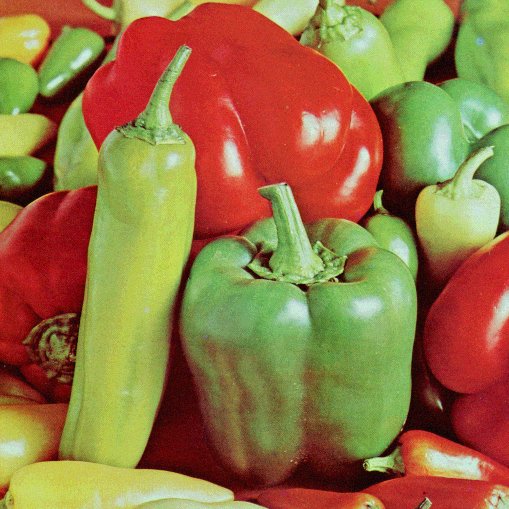
\includegraphics[width=1\textwidth]{peppers/peppers-48.png}
        \caption*{48\,\% (373\,kB)}
      \end{minipage}
    };
    \node [below=0.5cm of original] (500kb) {
      \begin{minipage}{0.35\textwidth}
        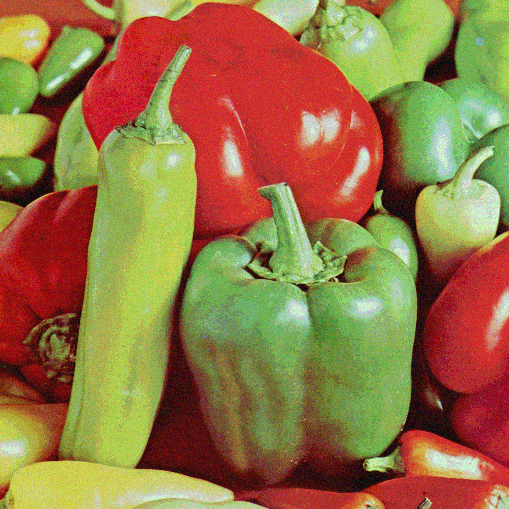
\includegraphics[width=1\textwidth]{peppers/peppers-60.png}
        \caption*{60\,\% (466\,kB)}
      \end{minipage}
    };
    \node [below=0.5cm of 300kb] (700kb) {
      \begin{minipage}{0.35\textwidth}
        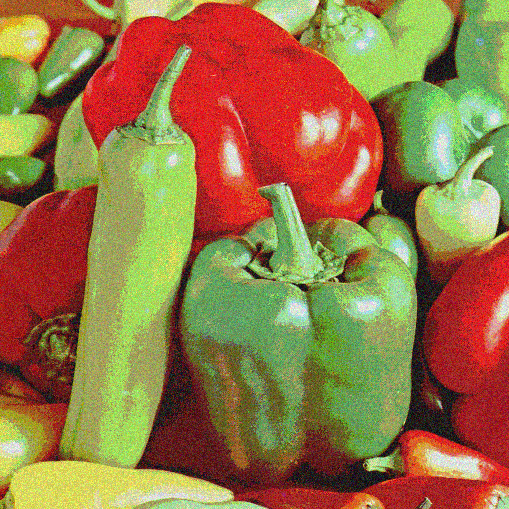
\includegraphics[width=1\textwidth]{peppers/peppers-72.png}
        \caption*{72\,\% (560\,kB)}
      \end{minipage}
    };

    \matrix [column sep=3.5cm] at ($(original.north)!0.5!(300kb.north) + (0,3.5cm)$) {
      \coordinate (a); & \coordinate (b); & \coordinate (c); & \coordinate (d); \\
    };

    \coordinate (spy-on) at (-0.95cm,-0.8cm);

    \spy on ($(original.north) + (spy-on)$) in node[label=below:Original] at (a);
    \spy on ($(300kb.north) + (spy-on)$) in node[label=below:48\,\%] at (b);
    \spy on ($(500kb.north) + (spy-on)$) in node[label=below:60\,\%] at (c);
    \spy on ($(700kb.north) + (spy-on)$) in node[label=below:72\,\%] at (d);


  \end{tikzpicture}
  \caption{Paprika mit einer Größe von 509 $\times$ 509 Pixel.
    Gute Bildqualität zwischen 373 und 466\,kB versteckter Nachricht ($\bmax \approx 777$\,kB).}
  \label{fig:example-peppers}
\end{figure}


\newpage

\begin{figure}[h!]
  \centering
  \begin{tikzpicture}
    [spy scope= {circle, magnification=8, size=3cm},
      every spy on node/.style={draw, Red, ultra thick},
      every node/.style={inner sep=0},
      label distance=-1cm]

    \node (original) {
      \begin{minipage}{0.45\textwidth}
        \includegraphics[width=1\textwidth]{turtle.png}
        \caption*{Original}
      \end{minipage}
    };
    \node [right= of original] (2mb) {
      \begin{minipage}{0.45\textwidth}
        \includegraphics[width=1\textwidth]{turtle-2000000.png}
        \caption*{2 MB Nachricht}
      \end{minipage}
    };
    \node [below=0.5cm of original] (4mb) {
      \begin{minipage}{0.45\textwidth}
        \includegraphics[width=1\textwidth]{turtle-4000000.png}
        \caption*{4 MB Nachricht}
      \end{minipage}
    };
    \node [below=0.5cm of 2mb] (6mb) {
      \begin{minipage}{0.45\textwidth}
        \includegraphics[width=1\textwidth]{turtle-6000000.png}
        \caption*{6 MB Nachricht}
      \end{minipage}
    };

    \matrix [column sep=3.5cm] at ($(original.north)!0.5!(2mb.north) + (0,3.5cm)$) {
      \coordinate (a); & \coordinate (b); & \coordinate (c); & \coordinate (d); \\
    };

    \coordinate (spy-on) at (1cm,-0.5cm);

    \spy on ($(original.north) + (spy-on)$) in node[label=below:Original] at (a);
    \spy on ($(2mb.north) + (spy-on)$) in node[label=below:2 MB] at (b);
    \spy on ($(4mb.north) + (spy-on)$) in node[label=below:4 MB] at (c);
    \spy on ($(6mb.north) + (spy-on)$) in node[label=below:6 MB] at (d);


  \end{tikzpicture}
  \caption{Schildkröte. Größe 1368 $\times$ 1824 Pixel. Maximale Kapazität $\approx 7,5$ MB.
    Gute Bildqualität bis zu 4MB versteckter Nachricht.}
  \label{fig:example-turtle}
\end{figure}


\newpage

\begin{figure}[h!]
  \centering
  \begin{tikzpicture}
    [spy scope= {circle, magnification=6, size=3cm},
      every spy on node/.style={draw, Red, thick},
      every node/.style={inner sep=0},
      label distance=-1cm]

    \node (original) {
      \begin{minipage}{0.45\textwidth}
        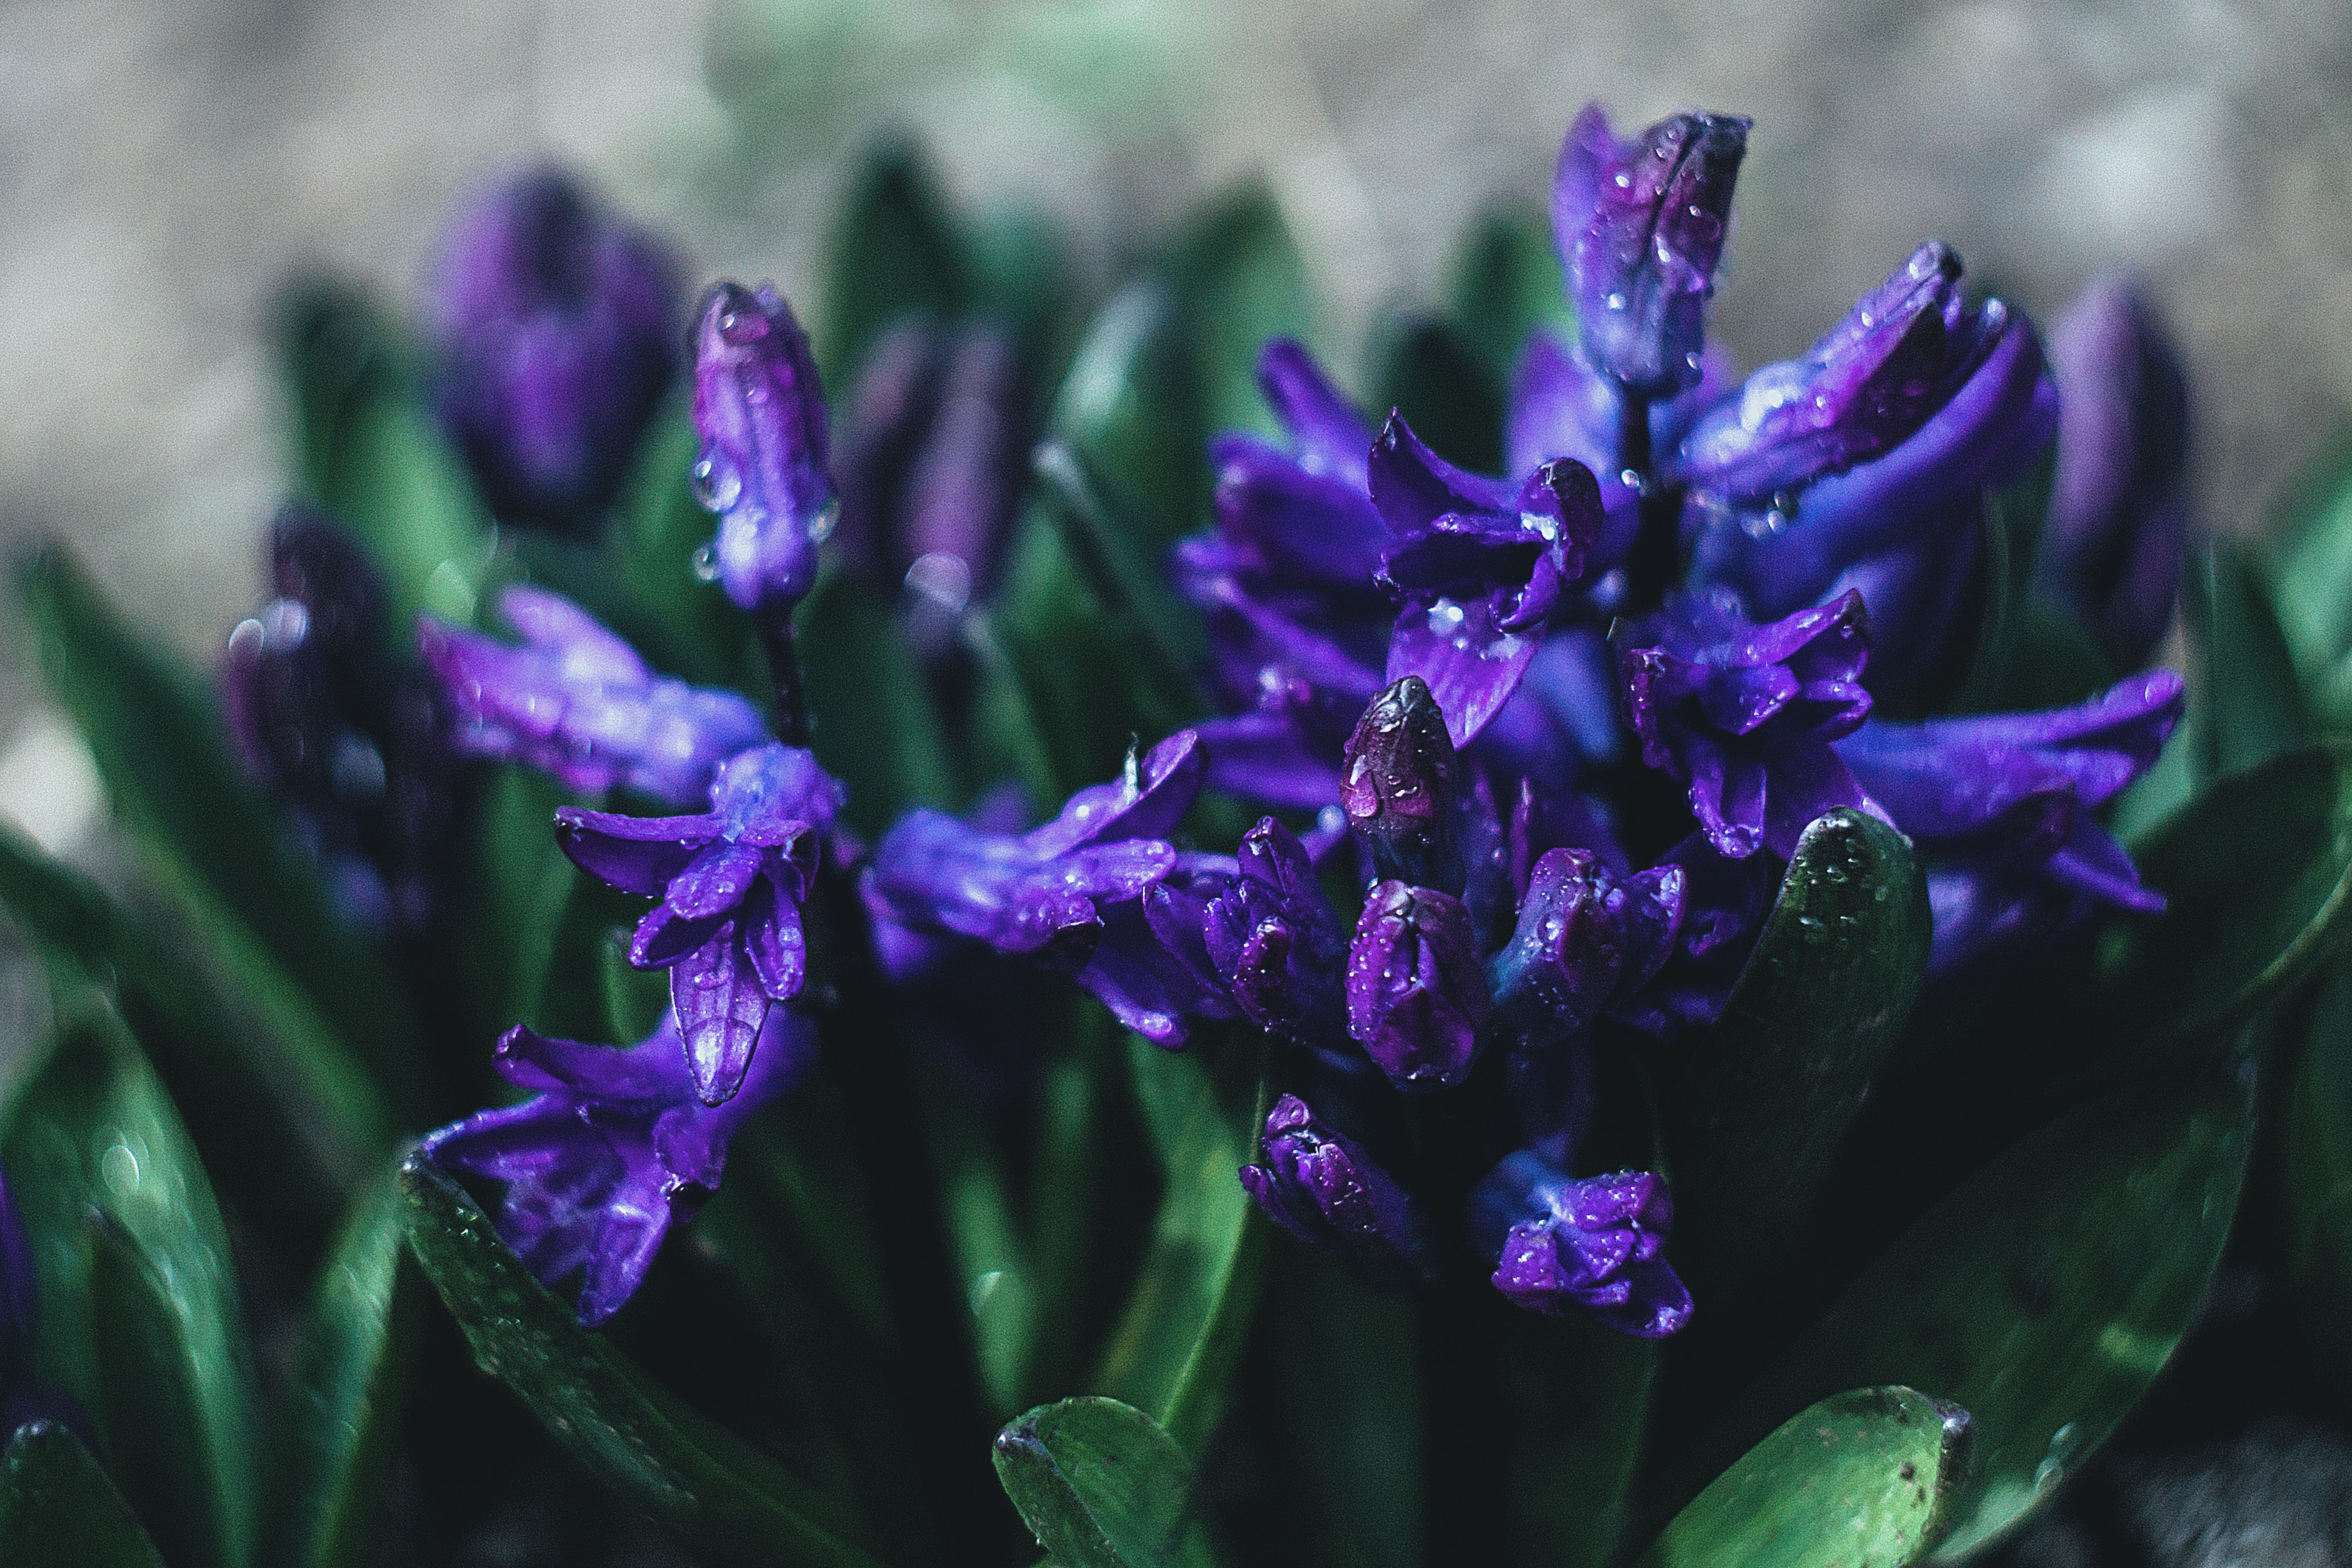
\includegraphics[width=1\textwidth]{flowers/flowers.png}
        \caption*{Original}
      \end{minipage}
    };
    \node [right= of original] (10mb) {
      \begin{minipage}{0.45\textwidth}
        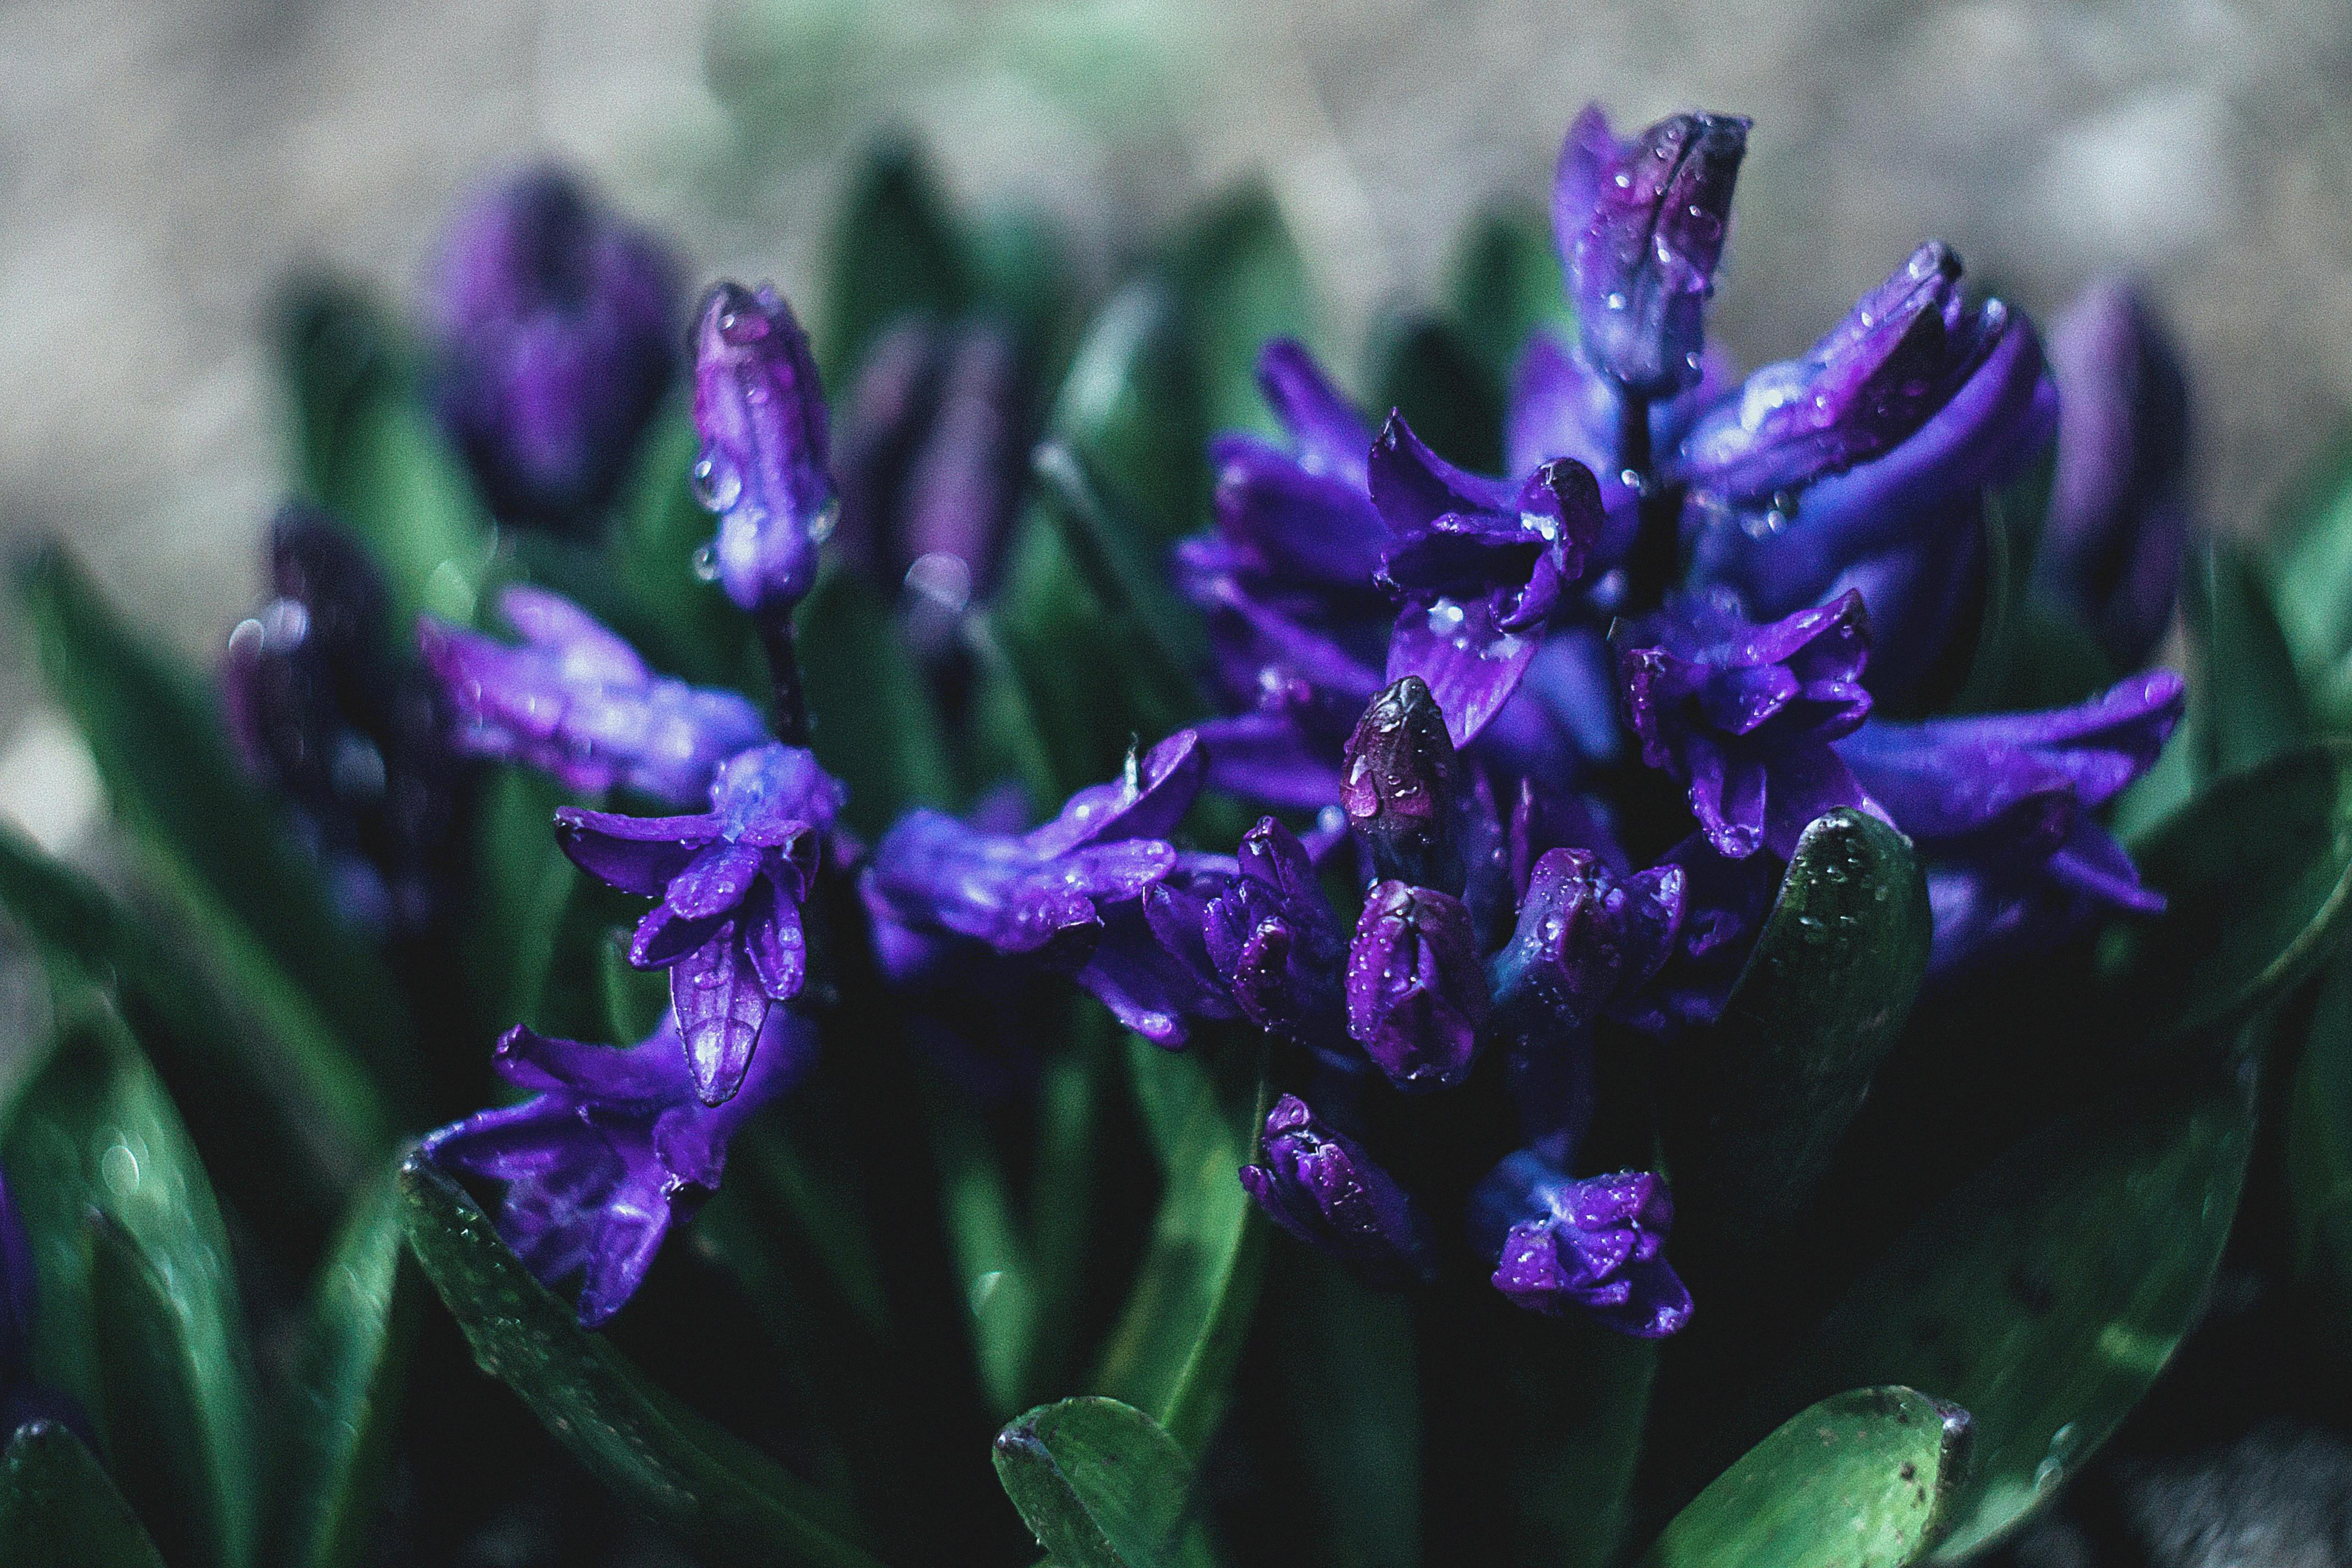
\includegraphics[width=1\textwidth]{flowers/flowers-48.png}
        \caption*{48\,\% (\num{17.5}\,MB)}
      \end{minipage}
    };
    \node [below=0.5cm of original] (20mb) {
      \begin{minipage}{0.45\textwidth}
        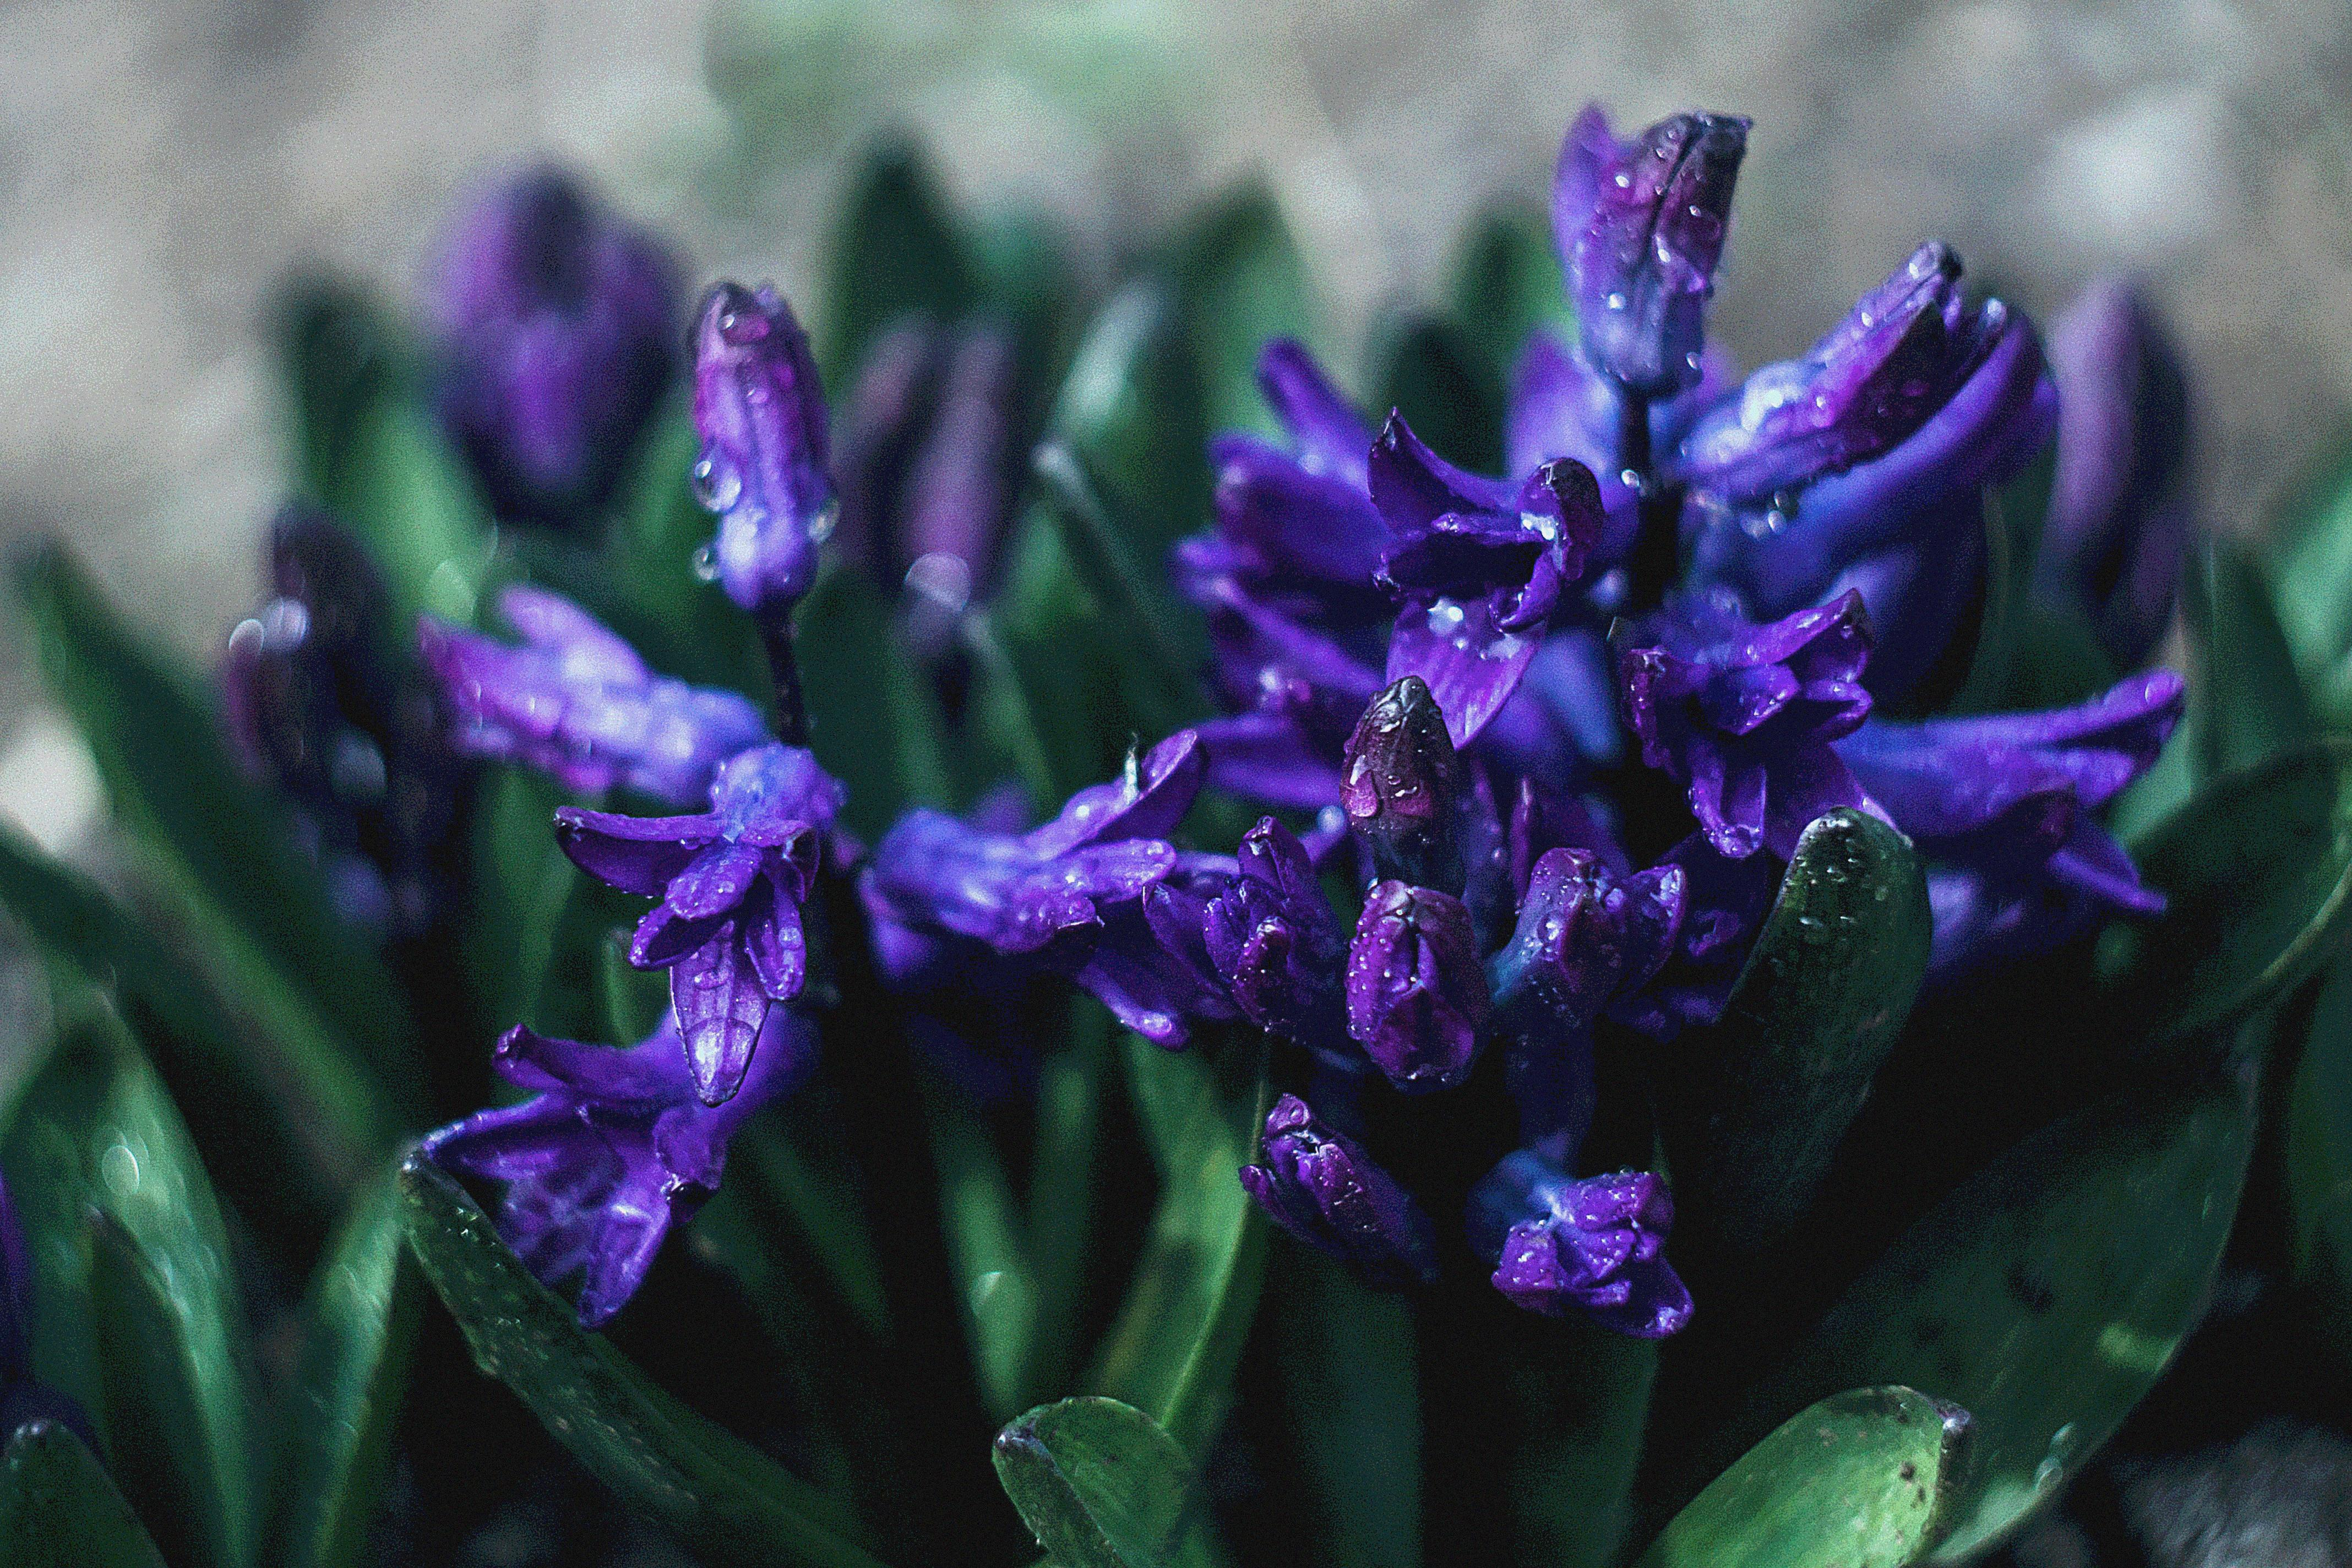
\includegraphics[width=1\textwidth]{flowers/flowers-60.png}
        \caption*{60\,\% (\num{21.9}\,MB)}
      \end{minipage}
    };
    \node [below=0.5cm of 10mb] (30mb) {
      \begin{minipage}{0.45\textwidth}
        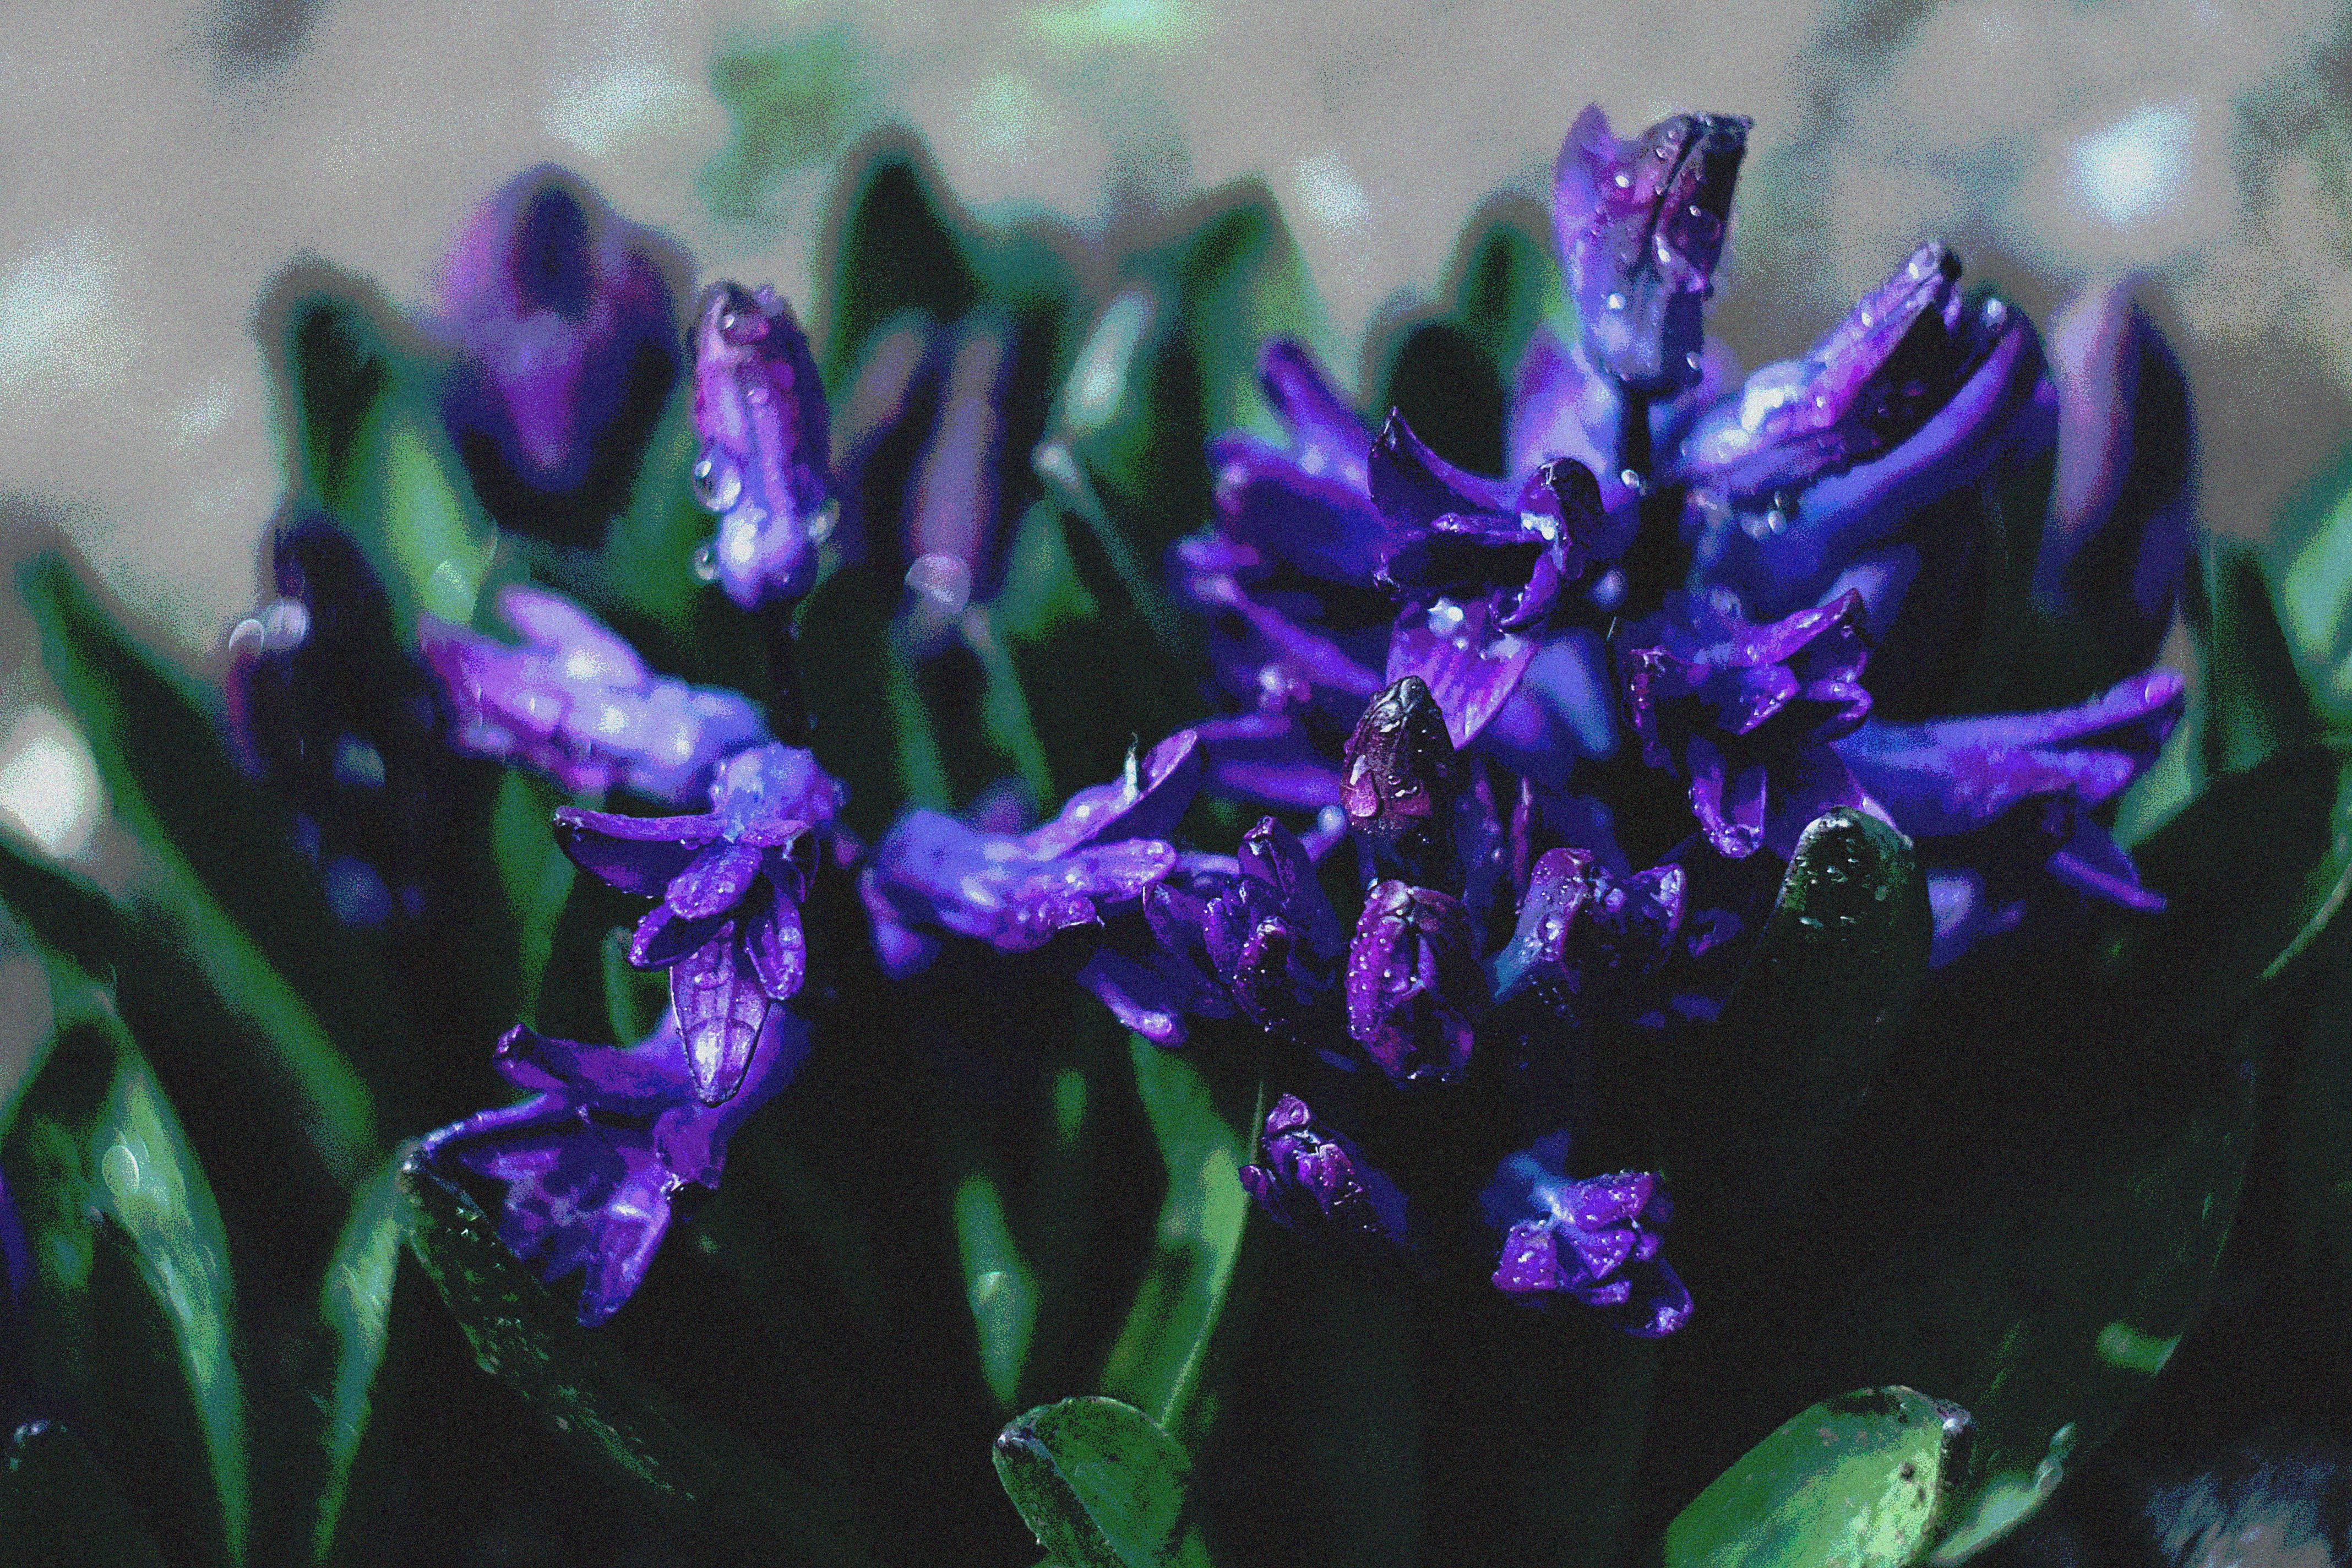
\includegraphics[width=1\textwidth]{flowers/flowers-72.png}
        \caption*{72\,\% (\num{26.3}\,MB)}
      \end{minipage}
    };

    \matrix [column sep=3.5cm] at ($(original.north)!0.5!(10mb.north) + (0,3.5cm)$) {
      \coordinate (a); & \coordinate (b); & \coordinate (c); & \coordinate (d); \\
    };

    \coordinate (spy-on) at (1.05cm,-0.55cm);

    \spy on ($(original.north) + (spy-on)$) in node[label=below:Original] at (a);
    \spy on ($(10mb.north) + (spy-on)$) in node[label=below:48\,\%] at (b);
    \spy on ($(20mb.north) + (spy-on)$) in node[label=below:60\,\%] at (c);
    \spy on ($(30mb.north) + (spy-on)$) in node[label=below:72\,\%] at (d);

  \end{tikzpicture}
  \caption{Blumen mit einer Größe von 2848 $\times$ 4272 Pixel.
    Gute Bildqualität bis zu 22\,MB versteckter
    Nachricht ($\bmax \approx \num{36.5}$\,MB).}
  \label{fig:example-flowers}
\end{figure}


\newpage





\section{Fazit und Ausblick}
Sind die Seitenverhältnisse eines Bilds Zweierpotenzen, entstehen Streifen,
welche einfacher erkannt werden können. \autoref{fig:example-white-stripes} zeigt dieses
Verhalten, die veränderte Pixel sind weiß eingefärbt.
\vspace{2cm}
\begin{figure}[h!]
  \centering
  
\includegraphics{black-white-stripes.png}
  \caption{Koordinatenverteilung auf einem $512 \times 512$ Pixel Schwarzbild
    für eine Nachrichtenlänge von 10 KB.}
  \label{fig:example-white-stripes}
\end{figure}